%%%%%%%%%%%%%%%%%%%%%%%%%%%%%%%%%%%%%%%%%
% Masters/Doctoral Thesis 
% LaTeX Template
% Version 2.5 (27/8/17)
%
% This template was downloaded from:
% http://www.LaTeXTemplates.com
%
% Version 2.x major modifications by:
% Vel (vel@latextemplates.com)
%
% This template is based on a template by:
% Steve Gunn (http://users.ecs.soton.ac.uk/srg/softwaretools/document/templates/)
% Sunil Patel (http://www.sunilpatel.co.uk/thesis-template/)
%
% Template license:
% CC BY-NC-SA 3.0 (http://creativecommons.org/licenses/by-nc-sa/3.0/)
%
%%%%%%%%%%%%%%%%%%%%%%%%%%%%%%%%%%%%%%%%%

%----------------------------------------------------------------------------------------
%	PACKAGES AND OTHER DOCUMENT CONFIGURATIONS
%----------------------------------------------------------------------------------------

\documentclass[
11pt, % The default document font size, options: 10pt, 11pt, 12pt
oneside, % Two side (alternating margins) for binding by default, uncomment to switch to one side
english, % ngerman for German
doublespacing, % Single line spacing, alternatives: onehalfspacing or doublespacing
%draft, % Uncomment to enable draft mode (no pictures, no links, overfull hboxes indicated)
%nolistspacing, % If the document is onehalfspacing or doublespacing, uncomment this to set spacing in lists to single
%liststotoc, % Uncomment to add the list of figures/tables/etc to the table of contents
%toctotoc, % Uncomment to add the main table of contents to the table of contents
%parskip, % Uncomment to add space between paragraphs
%nohyperref, % Uncomment to not load the hyperref package
headsepline, % Uncomment to get a line under the header
chapterinoneline, % Uncomment to place the chapter title next to the number on one line
%consistentlayout, % Uncomment to change the layout of the declaration, abstract and acknowledgements pages to match the default layout
]{MastersDoctoralThesis} % The class file specifying the document structure

\usepackage[utf8]{inputenc} % Required for inputting international characters
\usepackage[T1]{fontenc} % Output font encoding for international characters

\usepackage{mathpazo} % Use the Palatino font by default

\usepackage[backend=bibtex, style=numeric, natbib=true, sorting=none]{biblatex} % Use the bibtex backend with the authoryear citation style (which resembles APA)

\addbibresource{QE_bib.bib} % The filename of the bibliography

\usepackage[autostyle=true]{csquotes} % Required to generate language-dependent quotes in the bibliography

\usepackage{etoolbox}
\makeatletter
\patchcmd{\chapter}{\if@openright\cleardoublepage\else\clearpage\fi}{}{}{}
\makeatother

%----------------------------------------------------------------------------------------
%	MARGIN SETTINGS
%----------------------------------------------------------------------------------------

\geometry{
	paper=a4paper, % Change to letterpaper for US letter
	inner=2cm, % Inner margin
	outer=2cm, % Outer margin
	bindingoffset=0cm, % Binding offset
	top=1.5cm, % Top margin
	bottom=1.5cm, % Bottom margin
	%showframe, % Uncomment to show how the type block is set on the page
}

%----------------------------------------------------------------------------------------
%	THESIS INFORMATION
%----------------------------------------------------------------------------------------

\thesistitle{Mutational Patterns in Founder Populations} % Your thesis title, this is used in the title and abstract, print it elsewhere with \ttitle
\supervisor{Dr. Simon \textsc{Gravel}} % Your supervisor's name, this is used in the title page, print it elsewhere with \supname
\examiner{} % Your examiner's name, this is not currently used anywhere in the template, print it elsewhere with \examname
\degree{Doctor of Philosophy} % Your degree name, this is used in the title page and abstract, print it elsewhere with \degreename
\author{Luke \textsc{Anderson-Trocm\'e}} % Your name, this is used in the title page and abstract, print it elsewhere with \authorname
\addresses{} % Your address, this is not currently used anywhere in the template, print it elsewhere with \addressname

\subject{Statistical Population Genetics} % Your subject area, this is not currently used anywhere in the template, print it elsewhere with \subjectname
\keywords{} % Keywords for your thesis, this is not currently used anywhere in the template, print it elsewhere with \keywordnames
\university{\href{http://www.mcgill.ca}{McGill University}} % Your university's name and URL, this is used in the title page and abstract, print it elsewhere with \univname
\department{\href{https://www.mcgill.ca/humangenetics/}{Department of Human Genetics}} % Your department's name and URL, this is used in the title page and abstract, print it elsewhere with \deptname
\group{\href{http://simongravel.lab.mcgill.ca/Home.html}{Gravel Lab}} % Your research group's name and URL, this is used in the title page, print it elsewhere with \groupname
\faculty{\href{https://www.mcgill.ca/medicine/}{Faculty of Medecine}} % Your faculty's name and URL, this is used in the title page and abstract, print it elsewhere with \facname

\AtBeginDocument{
\hypersetup{pdftitle=\ttitle} % Set the PDF's title to your title
\hypersetup{pdfauthor=\authorname} % Set the PDF's author to your name
\hypersetup{pdfkeywords=\keywordnames} % Set the PDF's keywords to your keywords
}

\begin{document}

\frontmatter % Use roman page numbering style (i, ii, iii, iv...) for the pre-content pages

\pagestyle{plain} % Default to the plain heading style until the thesis style is called for the body content

%----------------------------------------------------------------------------------------
%	TITLE PAGE
%----------------------------------------------------------------------------------------

\begin{titlepage}
\begin{center}


\includegraphics[width=40mm]{./Figures/McGill.png} % University/department logo

\vspace*{.06\textheight}
{\scshape\LARGE \univname\par}\vspace{1.5cm} % University name
\textsc{\Large Qualifying Exam}\\[0.5cm] % Thesis type

\HRule \\[0.4cm] % Horizontal line
{\huge \bfseries \ttitle\par}\vspace{0.4cm} % Thesis title
\HRule \\[1.5cm] % Horizontal line
 
\begin{minipage}[t]{0.4\textwidth}
\begin{flushleft} \large
\emph{Author:}\\
{\authorname} % Author name - remove the \href bracket to remove the link
\end{flushleft}
\end{minipage}
\begin{minipage}[t]{0.4\textwidth}
\begin{flushright} \large
\emph{Supervisor:} \\
{\supname} % Supervisor name - remove the \href bracket to remove the link  
\end{flushright}
\end{minipage}\\[3cm]

\deptname\\\facname\\[2cm] % Research group name and department name

{\large \today}\\[4cm] % Date

\vfill
\end{center}
\end{titlepage}


%----------------------------------------------------------------------------------------
%	THESIS CONTENT - CHAPTERS
%----------------------------------------------------------------------------------------

\mainmatter % Begin numeric (1,2,3...) page numberingc
\pagestyle{thesis} % Return the page headers back to the "thesis" style

\newgeometry{
	paper=a4paper, % Change to letterpaper for US letter
	inner=2cm, % Inner margin
	outer=2cm, % Outer margin
	bindingoffset=0cm, % Binding offset
	top=3cm, % Top margin
	bottom=1.5cm, % Bottom margin
	%showframe, % Uncomment to show how the type block is set on the page
}
	
\section{Introduction}
The human genome is composed of a mosaic of ancestral genetic material that has been passed on for millennia.
This pattern of interconnected relatedness is beginning to unveil humanity's rich and complex history.
For example, sequence data estimates that Human expansion out of Africa (OOA) occurred between 45,000 and 60,000 years ago \citep{Henn2012}. 
As humans expanded into new habitats, each new colony was founded by a smaller group departing a larger, more diverse source population.
The impacts of the OOA bottleneck are still measurable, as distance from Africa is strongly correlated with decreasing genetic diversity \citep{Ramachandran2005}.

Bottlenecks can drastically change the allele frequencies within a population and lead to rapid divergences \citep{Rosenberg2002, Charlesworth2003, Balick2015}.
Rare alleles in the source population can increase significantly in frequency or even become fixed in the founder population.
Isolation over time can lead to increased diversity between small populations, while the diversity within may remain relatively low. 
For this reason, migration between populations can increase the genetic diversity of both populations \citep{Charlesworth2003}.

Recent events of admixture are tractable with genomic analyses like identity by descent (IBD) mapping and coalescence estimations \citep{Baharian2016}.
However, recombination over time will fragment haplotypes eventually making it difficult to determine their ancestry.
Despite this, a population will retain a unique set of alleles at frequencies waxing and waning over time.
These allele frequencies can then be used to estimate demographic histories of multiple populations \citep{Gravel2011}. 

Many disease or phenotype association tests are susceptible to spurious results caused by population structure.
In order to properly account for this, a better understanding of human demographic history is needed \citep{Gravel2011}.
Moreover, studying recent founder populations can lead to a better understanding of the mechanisms and dynamics of historical founder events. 

\subsection{Thesis proposal}
The aim of this PhD project is to study the genomics of founder populations to infer population specific mutational signatures, demographic history and mutation rates.
\textbf{Our hypotheses are}: 

\textbf{1}. Using higher quality data can clarify the nature of the mutational pattern observed in Japan. Alternatively, the mutational pattern may be a technical artifact unique to the original data.

\textbf{2}. The heterogeneity of Quebec's population structure can be accounted for both by a series of founder events and ancestral population structure predating the colonization of Canada.

\textbf{3}. Leveraging phylogenetic records in combination with sequence data can improve the estimates of mutation rates.
\vfill
\restoregeometry 
\chapter{Mutational signatures in Japan}

\subsection{Batch Effects in Aging Reference Cohort Data}	
The last 5 years have seen a drastic increase in the amount and quality of human genome sequence data. 
Reference cohorts such as the International HapMap Project \citep{HapMap2005}, the 1000 Genomes Project \citep{1000GenomesProjectConsortium2010,The1000GenomesProjectConsortium2012}, and the Simons Diversity project \citep{Mallick2016}, for example, have made thousands of genome sequences publicly available for population and medical genetic analyses. 
Many more genomes are available indirectly through servers providing imputation services \citep{HapMap2005} or summary statistics for variant frequency estimation \citep{Lek2016}.

The first genomes in the 1kGP were sequenced 10 years ago \citep{VanDijk2014}. 
Since then, sequencing platforms have rapidly improved. 
Yet, because of the extraordinary value of freely available data, early data from the 1000 Genomes project (1kGP) is still widely used as a reference panel for imputation, allele frequency estimations and to answer a wide range of medical and evolutionary questions. 
The second phase of the 1kGP implemented multiple technological and analytical improvements over its earlier phases \citep{The1000GenomesProjectConsortium2012}, leading to heterogeneous sample preparations and data quality.

Even though such batch effects clearly have the potential to confound analyses, the usefulness and ubiquity of the 1kGP data make such issues particularly insidious.   
This raises the question of whether and how such legacy data should be included in contemporary analyses alongside more recent cohorts.
Here we point out how large and previously unreported batch effects in the early phases of the 1kGP still lead to incorrect genetic conclusions through population genetic analyses and indirect use through prominent imputation servers.

\subsection{Mutational Signatures}
There has been recent interest in population variation in germline mutational signatures which can be revealed in large sequencing panels. 
In 2015, Harris reported 50\% more TCC ${\rightarrow}$ TTC mutations in European populations compared to African populations, and this was replicated in a different cohort in 2017 \citep{Harris2015a, Harris2017a, Mathieson2017a}. 
Strong population enrichments of a mutational signature suggest important genetic or environmental differences in the history of each population \citep{Harris2015a, Harris2017a}. 
Harris and Pritchard further identified distinct mutational spectra across a range of populations, which were further examined in a recent publication by Aikens et al. \citep{Harris2017a,Aikens2018}.
 
In particular, both studies  identified a heterogeneous mutational signature within 1000 Genomes Project (1kGP) Japanese individuals.
This heterogeneity is intriguing because differences in germline signatures accumulate over many generations.
A systematic difference within the Japanese population would suggest sustained environmental or genetic differences across sub-populations within Japan with little to no gene flow.
We therefore decided to follow up on this observation, by using a newly sequenced dataset of Japanese individuals. 

\section{Results}
\subsection{A peculiar mutational signature in Japan}
Harris and Pritchard reported an excess of a 3-mer substitution patterns *AC${\rightarrow}$*CC in a portion of the Japanese individuals in the 1kGP \citep{Harris2017a}.
While trying to follow up on this observation in a larger and more recent Japanese cohort, we did not find this particular signature.
When comparing the allele frequencies between the Japanese individuals from the 1kGP and this larger dataset, we observed a number of single nucleotide polymorphisms (SNPs) private to one of the two groups (Figure \ref{SFS}).
Given the similarity of the two populations, this strongly suggests a technical difference rather than a population structure effect.
These mismatches were maintained after filtering for low-quality regions of the human genome and sites failing Hardy-Weinberg equilibrium tests.
\subsection{Reverse GWAS}
To identify SNPs that are likely to reproduce poorly across cohorts without having access to a second cohort, we performed an association study on the Japanese from the 1kGP (JPT) for variants that associate strongly with low average quality of mapped bases ($Q$) (Figure \ref{SFS}).
Traditionally, genome wide association studies use genotypes as the independent variable. 
Here we perform a "reverse GWAS", in the sense that genotypes are now the dependent variable that we attempt to predict using the continuous variable $Q$ as the independent variable.
We use logistic regression of the genotypes on $Q$ and identify 587 SNPs with $p < 10^{-8}$ and 1034 SNPs with $ p < 10^{-6}$.

\subsection{Identifying Suspicious SNPs in the 1kGP}
The distribution of $Q$ across 1kGP populations shows that many populations have distributions of $Q$ scores comparable to that of the JPT, especially populations sequenced in the phase 1 of the project: sequencing done in the early phases of the 1kGP was more variable and overall tended to include lower quality sequencing data (Figure \ref{MapQual}).
This variability could result from evolving sequence platform and protocols or variation between sequencing centres. 
By 2011, older sequencing technologies were phased out, and methods became more consistent, resulting in higher and more uniform quality.
We performed the reverse GWAS approach in all populations and identified 3826 variants that were independently associated to low $Q$ in at least two populations with $ p < 10^{-6}$ (Figure \ref{OverLap}). 

\subsection{Suspicious variants impact modern genomics analyses}
We searched the literature for any GWAS that might have reported these dubious variants as being significantly associated with some biological trait, even though there is no particular reason for these SNPS to be associated with phenotypes.
The NHGRI-EBI Catalog of published genome-wide association studies identified three recent publications that had reported these variants as close to or above the genome-wide significant threshold.
Two of these studies genotyped individuals and imputed the data using the HapMap II as a reference  database for imputation \citep{Kraja2011, Ebejer2013}.
The third study used the 1kGP sequence data and cell lines directly \citep{Mandage2017}.
Despite using state-of-the-art quality controls, these erroneous variants managed not only to be imputed onto real genotype data, but they also nearly reached genome wide significance for biological traits.

The HapMap project and 1kGP shared some cell lines but used different sequencing platforms to produce the data.
It is possible that a cell line artifact may have produced the same suspicious SNPs in the two sequencing projects.

\section{Conclusion}
The genome wide simple logistic regression analysis approach is rather straightforward, and could be a standard in a variety of -omics studies.
Given rapid technological progress, the focus of genomic research is naturally on the data generation side. 
However, cleaning up data is also important to avoid generating spurious results. 
The present findings suggest that a substantial fraction of the final release of the 1kGP project is overdue for removal or re-sequencing. 
\vfill

\chapter{Population structure of Quebec}

\section{Brief history of Quebec}
The French-Canadian population of Quebec was founded over four centuries ago from \textasciitilde 8500 settlers from France \citep{Bherer2011,Laberge2005}.
This small number of settlers are the direct ancestors of the majority of Quebec's population of 7 million.
Moreover, ancestral contributions of these settlers across the Saint-Lawrence valley is uneven, whereby two thirds of the modern gene pool is attributed to the first 2600 founders \citep{Gagnon2001, Laberge2005}.
While the rates of consanguineous unions in Quebec were not higher than in Europe, small population sizes and isolation over time led to increased distant consanguinity \citep{Laberge2005}.

The North-East of Quebec is characterized historically as being more isolated with lower immigration rates compared to Western Quebec.
Saguenay-Lac-Saint-Jean and Charlevoix also display higher rates of some rare genetic diseases as well as increased homozygosity compared to Western Quebec \citep{Gagnon2001}.
Variation of disease prevalence across the Saint-Lawrence valley indicate that population structure varies across geographic regions \citep{Gagnon2001}.
Indeed, this pattern of genetic diversity is attributed to a number of factors like variation in native ancestry, geographic isolation and concentration of founders.\citep{Gagnon2001,Laberge2005,Bherer2011}.

The founders of Quebec are not all from the same regions in France.
In the seventeenth-century, while France consisted of a network of small densely populated towns, there were not many marriages across great distances \citep{Laberge2005}.
Thus, the French settlers from regions around Paris and Atlantic port towns provide initial population structure \citep{Laberge2005}.
Another source of genetic diversity in the French-Canadian population is an estimated 1\% Native American ancestry \citep{Moreau2013}.

\subsection{A case study of founder populations}

Many populations experienced founder effects as humans expanded out of Africa and populated the other continents.
Studying examples of founder effects in human populations is a great way to improve our understanding of human demographic histories.
The Quebec population is an good case study for population genetics for multiple reasons.
The source population of this bottleneck is still present, which may not be the case for more ancient migration events. 
Comparing allele frequencies between France and Quebec can determine more accurately the nature of the colonization.
The French-Canadian population also has deep genealogical records that span four centuries and includes over 3 million entries.
Quebec is not the only recent founder population, but it is among the largest and in combination with its rich genealogical records, it makes it an excellent cohort to study the impact of founder events \citep{Larmuseau2013,Bherer2011,Gagnon2001,Roy-Gagnon2011}.

\subsection{Previous studies of Quebec population structure}
There have been several studies in the past few decades that have examined the population structure of Quebec.
By analyzing the genealogical data they described distinct sub-populations and inferred the relative contribution of founders \citep{Gagnon2001, Bherer2011}.
Genotype data used to analyze linkage disequilibrium and homozygosity has also revealed significant structure measurable today \citep{ Roy-Gagnon2011}.
Quebec is not a homogeneous population, but rather made up of a combination of distinct sub-populations.
This was confirmed with Fst statistics of these groups, indicating substantial genetic structure \citep{Roy-Gagnon2011}.
Roy-Gagnon (2011) also reported that there was greater differentiation between sub-populations of Quebec than between European populations.
While this study included 140 genotyped individuals - a small sample by today's standards - they postulate that this difference is accounted for by genetic drift.
Alternatively, the heterogeneity of the founder effect in the Quebec population could be explained by a series of separate founder events influenced by variation in the relative isolation, and migration between settlements \citep{Gagnon2001,Laberge2005}.

\section{Materials and Methods}
\subsection{Genetic and genealogical data}
While the deep genealogical data has been studied for over a decade, linking the genealogy to genetic data has only been done with relatively small sample sizes \citep{Gagnon2001,Roy-Gagnon2011}.
The aim of the second chapter of this thesis will be to examine the genetic structure of the Quebec population using more recent and larger genomic datasets in combination with the deep genealogical and geographical data. 
Recently developed methodologies will also be of use to further characterize this genomic landscape.

We plan on using two main cohorts for this chapter. 
The Genizon cohort has 9961 samples from Quebec, genotyped on a variety of chips.
While this data has yet to be published, our first contribution has been cleaning and processing these data to account for the different genotyping chips used.
One key advantage of using this cohort is that we already linked 516 individuals to the BALSAC genealogical records.
We will also include data from the Cartagene project which will soon have over 12,000 genotyped Quebecers.

The BALSAC database is a genealogical tree of predominantly French-Canadian Quebecers.
It was compiled from birth, marriage and death certificates from the Catholic Church.
Because of the major role the Church played in French-Canadian society, these records are remarkably detailed and comprehensive.

\subsection{Test statistics : founder effect or ancient population structure?}
Using Fst statistics we can infer the relative differences between sub-populations of Quebec (see \citep{Roy-Gagnon2011}).
Dominic Nelson, a graduate student from the Gravel lab, has written software that can produce single locus forward simulations of the Quebec population using the genealogical data from BALSAC.
These simulations can be used to produce estimated differences between sub-populations resulting purely from a founder effect.
Comparing the Fst statistics between the real data and simulations will allow us to partition the variation as the result of preserved genetic structure from France or of drift from founder events.

\section{Preliminary results}

\subsection{Visualizing population structure}
In collaboration with another graduate student from the Gravel lab, Alex Diaz-Papkovich, we performed a UMAP projection of the Genizon genotype data \citep{mcinnes2018umap,diaz2018}.
This method takes the first $n$ principal components of genetic data as input ($n = 20$ in this case) and reduces this high dimensional data to a lower dimension that preserves the high dimensional topology.
UMAP has been shown to outperform dimension reduction techniques like tSNE both computationally and at preserving both local and global population structure \citep{diaz2018, mcinnes2018umap}.
This visualization of Quebec population structure shows five clusters which is in agreement with previous works (Figure \ref{UMAP}) \citep{Gagnon2001, Bherer2011,Roy-Gagnon2011}. 
\vfill
\subsection{The geography of genetics}
The three dimensional coordinates of the UMAP space (X,Y,Z) were converted to three dimensional color space (R,G,B) (Figure \ref{UMAP}).
Therefore, Individuals with similar color are closer to each other in the projection and presumably share more recent ancestry.
To link the genetic data to geographic coordinates, we used the marriage locations of the ancestors of those linked to the BALSAC database.
The ancestral locations of these individuals in combination with the three dimensional UMAP coloring scheme show geographic clustering of the five sub-populations.
This is in agreement with what Roy-Gagnon observed \citep{Roy-Gagnon2011}.
These preliminary results are very promising as they appear to capture the geographic and genetic clustering of the French-Canadian population of Quebec.

\section{Goals}
While Fst gives a good estimate of genome wide past coalescent rates, we plan on analyzing IBD segments as they can provide us with more detailed insight of demographic history \citep{Charlesworth2003, Ralph2013, Baharian2016}.
Because Fst takes in all polymorphisms as input for the statistic, it does not distinguish between recent and more ancient common ancestry \citep{Ralph2013}.
Analysis of IBD segments shared among individuals from Quebec can be useful for reconstructing the recent structure of relatedness.
The length of the shared segments can be used to estimate the number of generations leading back to a common ancestor \citep{Palamara2015,Campbell2012,Baharian2016}.
Combining this with geographical data can infer patterns of shared ancestry across the Saint-Lawrence valley.
Ralph (2013) identified a general trend of decreasing recent common ancestry with geographic distance as well as distinct regional signals of IBD in different European populations \citep{Ralph2013}.
Europe has a rich history of complex migratory patterns and demographic histories that is difficult to trace back with certainty. 
Quebec on the other hand has a much more recent history that may be easier to trace with IBD analysis.

While studying the French-Canadian populations on their own can provide a detailed historical inference of demographics, including samples from other European populations can provide more context.
We plan on expanding the current analyses to include data from French individuals which could be used to confirm the results from the Fst analysis as well as provide insight into which regions in France are source populations to regions in Quebec.
If our hypothesis is correct, we expect French data projected onto the preserved embeddings from Figure \ref{UMAP} to cluster with the distinct sub-groups of Quebec.
Dr. Christian Dina in the University of Nantes in France has expressed interest in sharing French genomics data for this project.

\newgeometry{
	paper=a4paper, % Change to letterpaper for US letter
	inner=2cm, % Inner margin
	outer=2cm, % Outer margin
	bindingoffset=0cm, % Binding offset
	top=2.6cm, % Top margin
	bottom=1.5cm, % Bottom margin
}
\chapter{Estimating human mutation rates}

\section{Review of current methods and limitations}

Mutation rate estimations are necessary for understanding the timing of evolutionary processes and events.
Neutral mutations are expected to arise at a constant rate in the genome, and can therefore be used as an evolutionary clock that can estimate divergence times \citep{Moorjani2016}. 
The basic equation of mutation rate is $\mu = N / LM$ where N is the number of mutations, L is the length of the region and M is the number of generations \citep{Narasimhan2016}.
Estimating mutation rates in humans has proven to be difficult for a number of reasons.
Mutation rates vary across the genome as some regions are more conserved than others. 
Mutation rates are also known to vary over time as shorter branches within the Ape family compared to other primates suggest a "hominoid rate slowdown" whereby mutation rates decreased in apes \citep{Moorjani2016, Scally2012}.
In addition, more recent studies have found that mutation rates can even vary among human populations. \citep{Harris2015a, Harris2017a}.

\subsection{Phylogenetic methods}
The first human mutation rates were estimated by Haldane (1935) using the rates of children born with rare diseases from unaffected parents \citep{Haldane1935}.
However, once sequence data became available, estimates were based on phylogenetic data and fossil records.
By using fossil record dating as an estimate for coalescence time $t$ and the sequence divergence $d$ between two species as the number of mutation that have occurred over that time span, mutation rates $\mu$ can be estimated as $\mu = 2d/t$ \citep{Scally2012}. 
Using this method with the time of divergence of Chimps and Humans of 6 to 10 million years, the mutation rates are estimated to be around $1\times10^{-9}$ up to $2.5\times10^{-8}$ \citep{Takahata1997, Scally2012, Moorjani2016, Narasimhan2016}.
The limitations of this approach are numerous, ranging from accuracy of fossil record dating, to estimating the average generation time for chimps and humans over millions of years.


\subsection{Direct methods}
Instead of using distant ancestry and fossil records, another more direct approach to estimating mutation rates is to sequence the genomes of parents and offspring. 
This approach tends to give estimates that are less than half of the rate compared to the phylogenetic approach ($1-1.25\times10^{-8}$) \citep{Shendure2015,Narasimhan2016}.
One issue with trio sequencing for mutation rates is that false-positive rates of sequencing technologies are difficult to account for considering how low the true mutation rate is.
Another issue is that the samples used for sequencing are not zygotes.
This leaves room for germline mosaicisms to artificially increase the number of mutations observed in a generation.

\subsection{Population genetics methods}
Methods for estimating mutation rates using population genetics are increasingly being used.
These approaches expand on the theory behind trio sequencing by including more distantly related individuals.
One approach involves autozygous segments observed in a founder population with a known pedigree \citep{Campbell2012}.
These segments shared by multiple individuals are compared and mutations in these segments are then used in combination with the number of generations separating two individuals \citep{Campbell2012}.
An estimated mutation rate of $1.2\times10^{-8}$ was obtained by using autozygous regions from 70 trio sequenced Hutterite families.
Palamara et al. (2015) describe an even more generalized method by identifying IBD segments from unrelated individuals and inferring the number of generations using coalescent theory \citep{Palamara2012,Palamara2015,Baharian2016}.
This method then regresses the number of mutations observed per base against the time of most recent common ancestor.
The slope of the regression is the mutation rate per generation and the intercept is the inferred genotyping false-positive rate.
Applying this method to 498 individuals from 250 families, they measured a mutation rate of ($2.08\times10^{-8}$)\citep{Palamara2015}.
%The major limitation to this method comes from the coalescence estimations.

\section{Goals}
The aim of the third chapter of this thesis will be to explore mutation rate estimations using a combination of sequence data and genealogical data from the French-Canadian population.
One preliminary objective might be to replicate the population genetics methods described above by Palamara et al. and Campbell et al. \citep{Palamara2015,Campbell2012}.
There remains much controversy over mutation rate estimations and applying each of these methods to the same dataset would be a useful comparison.

Considering the deep genealogical records available for the French-Canadian population, we may be able to improve on the Palamara method by acquiring more precise estimates of generation time separating two IBD segments.
Indeed, by linking individuals to the phylogenetic tree of the Quebec population, we may be able to better estimate the most recent common ancestor for a given segment of the genome.
In addition, we expect French-Canadians to share long IBD segments as a result of the relatively recent bottleneck, which increases the power for this method.
Furthermore, by grouping IBD segments according to genomic regions (e.g. coding, CpG islands, etc.) and running the analysis separately would provide us with a more detailed view of the genome wide mutation rate in humans.

\restoregeometry 
%----------------------------------------------------------------------------------------
%	THESIS CONTENT - APPENDICES
%----------------------------------------------------------------------------------------
\clearpage
\appendix % Cue to tell LaTeX that the following "chapters" are Appendices

\begin{figure}
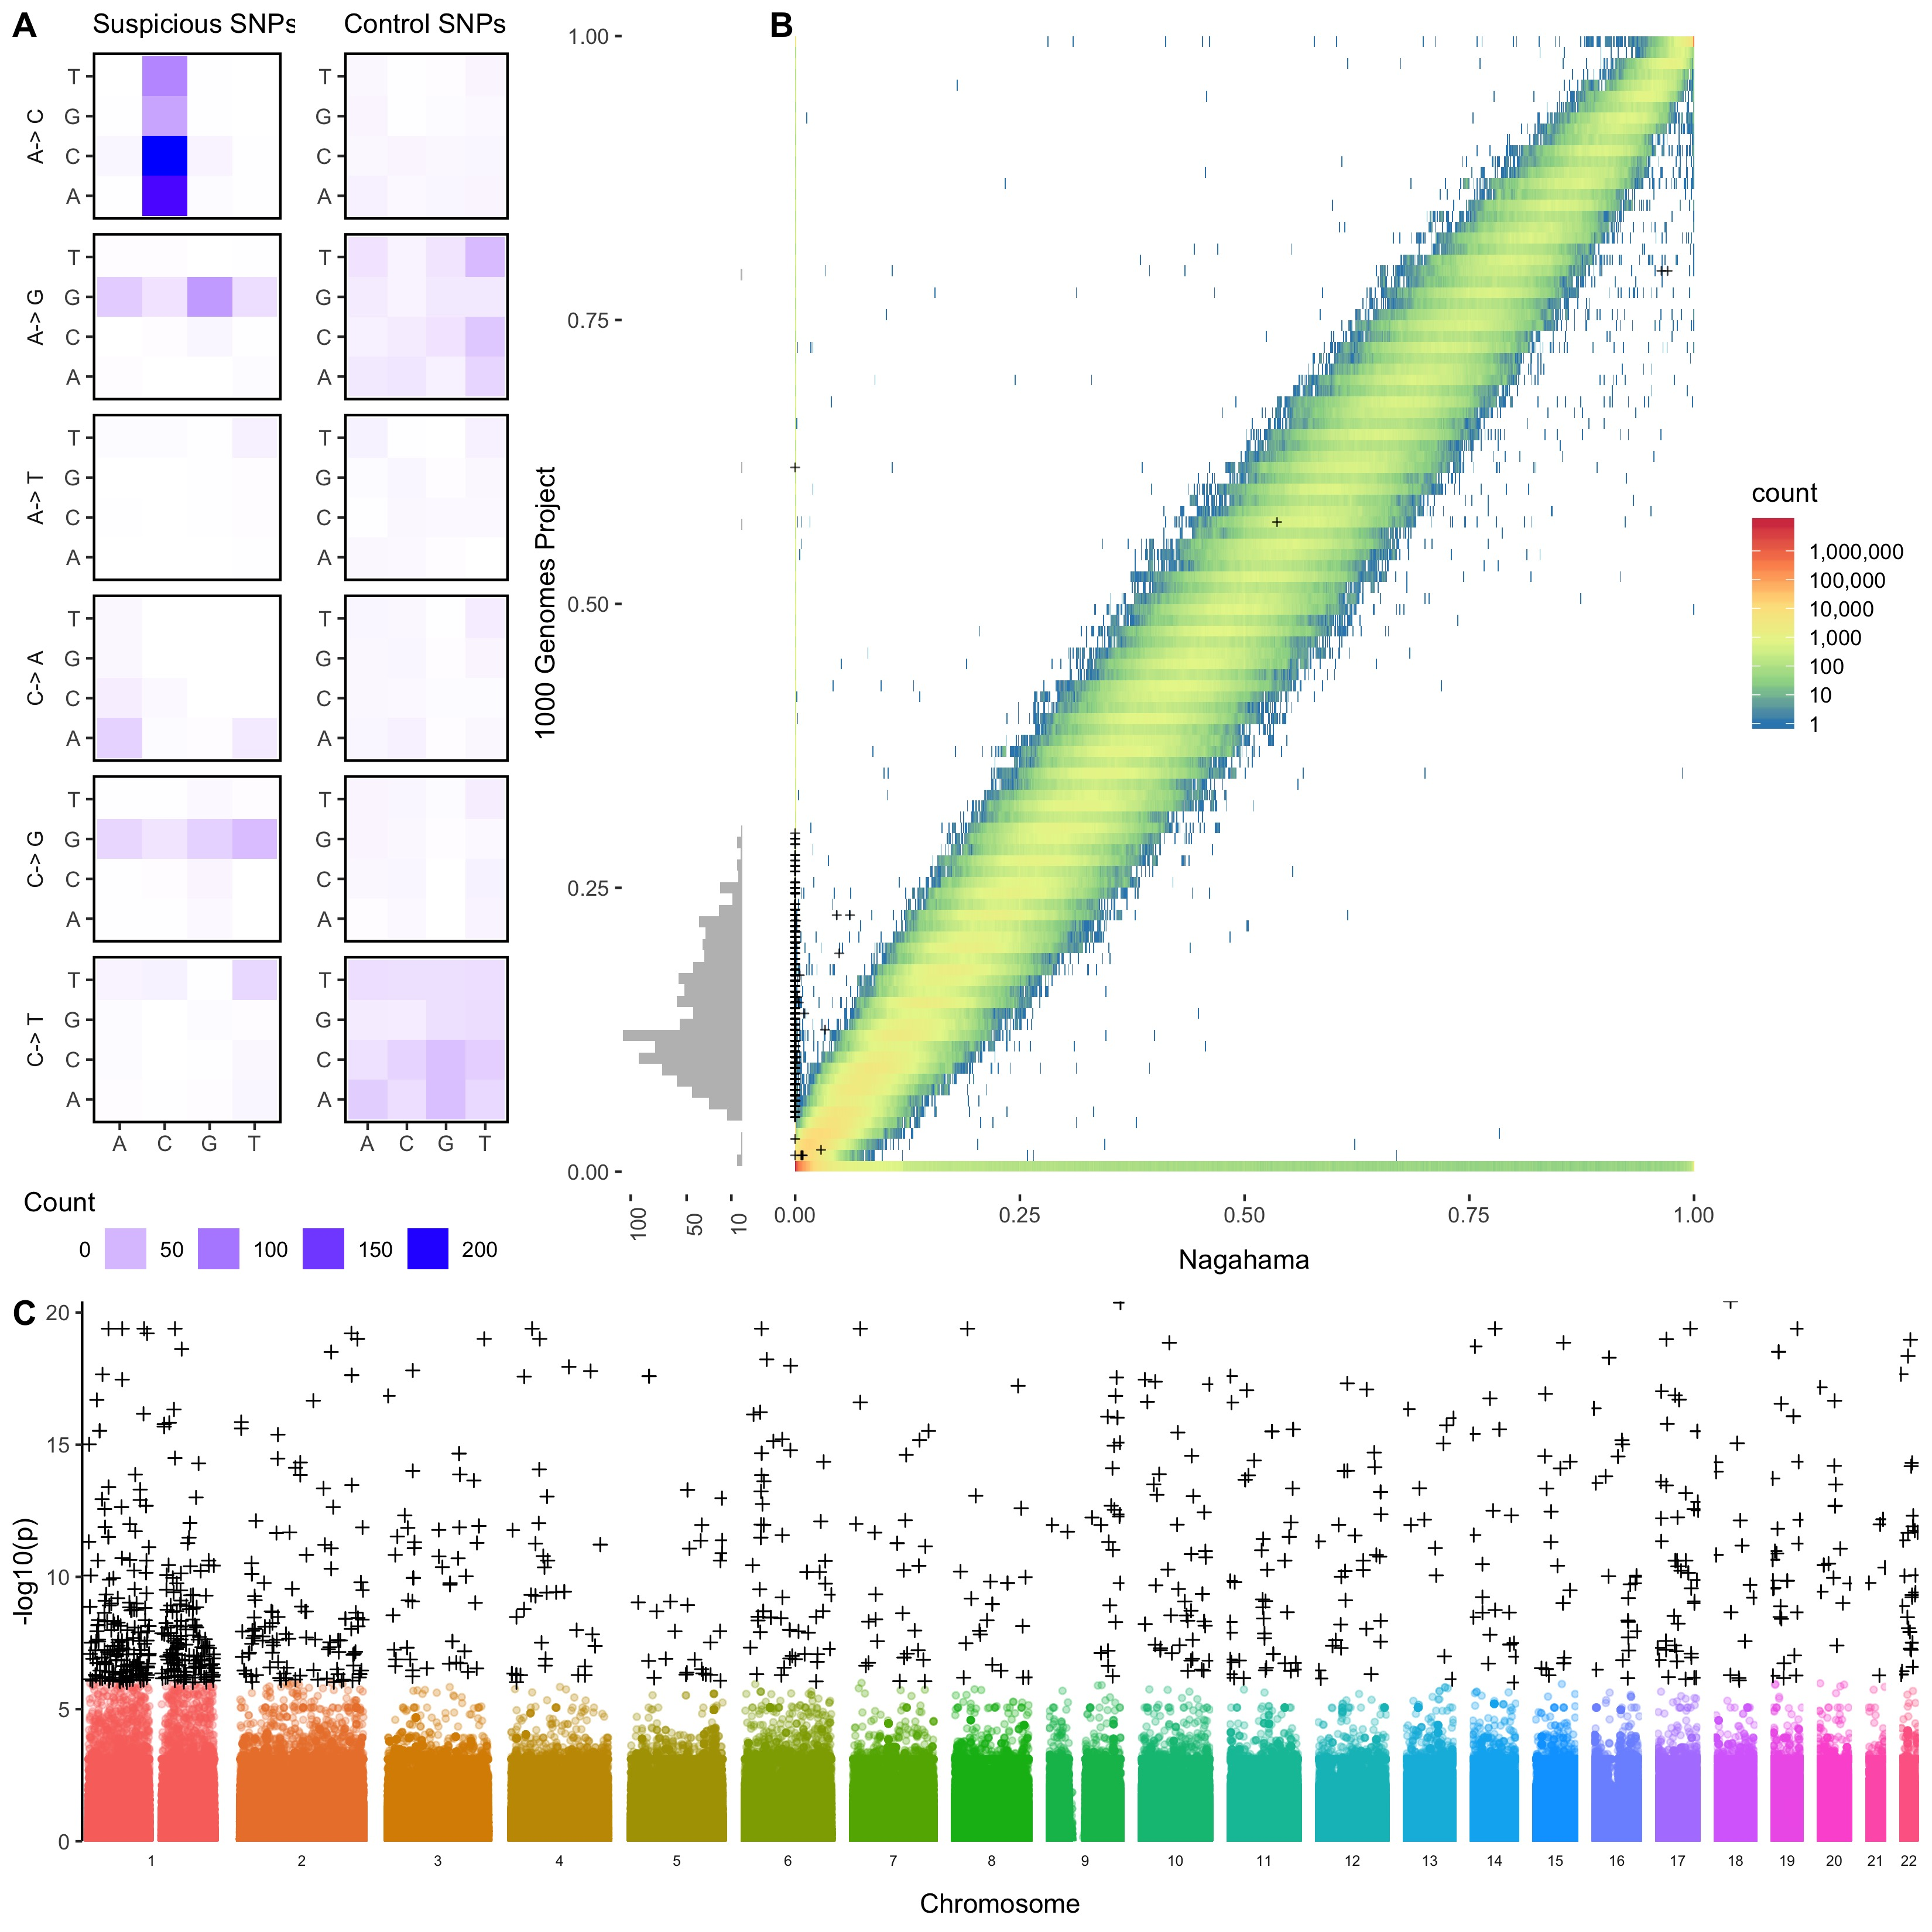
\includegraphics[width=\hsize,keepaspectratio]{./Figures/Figure1.jpg}
\caption{
\textbf{A} 
Mutation spectrum of the 1034 variants that reached a genome wide significance with a \textit{p}-value less than $p < 10^{-6}$  in a GWAS of sequencing quality. 
The majority of the variants with significant associations to $Q$ have the *AC${\rightarrow}$*CC mutational pattern. There is also a slight enrichment in GA*${\rightarrow}$GG* and GC*${\rightarrow}$GG* mutations. These three enrichments can be summarized as G**${\rightarrow}$GG*. (note: the reverse complement of *AC${\rightarrow}$*CC is GT*${\rightarrow}$GG*)
\textbf{B} 
Joint frequency spectrum plot of the Japanese from the 1kGP and a more recent Nagahama dataset.
Crosses ( + ) are variants that reached genome wide significance in a GWAS of sequencing quality. 
The histogram on the left of the plot is the distribution of significant variants. 
\textbf{C} 
Genome wide association of the average quality of mapped bases $Q$ for the 104 Japanese individuals included in the 1kGP. This GWAS identified $587\ \  p < 10^{-8}$ and $1034\ \ p < 10^{-6}$ SNPs that were associated to the average $Q$ of SNPs mapped for an individual
The same analysis was performed independently for each of the populations in the 1kGP. }
 \label{SFS}
\end{figure}

\begin{figure}
\begin{center}
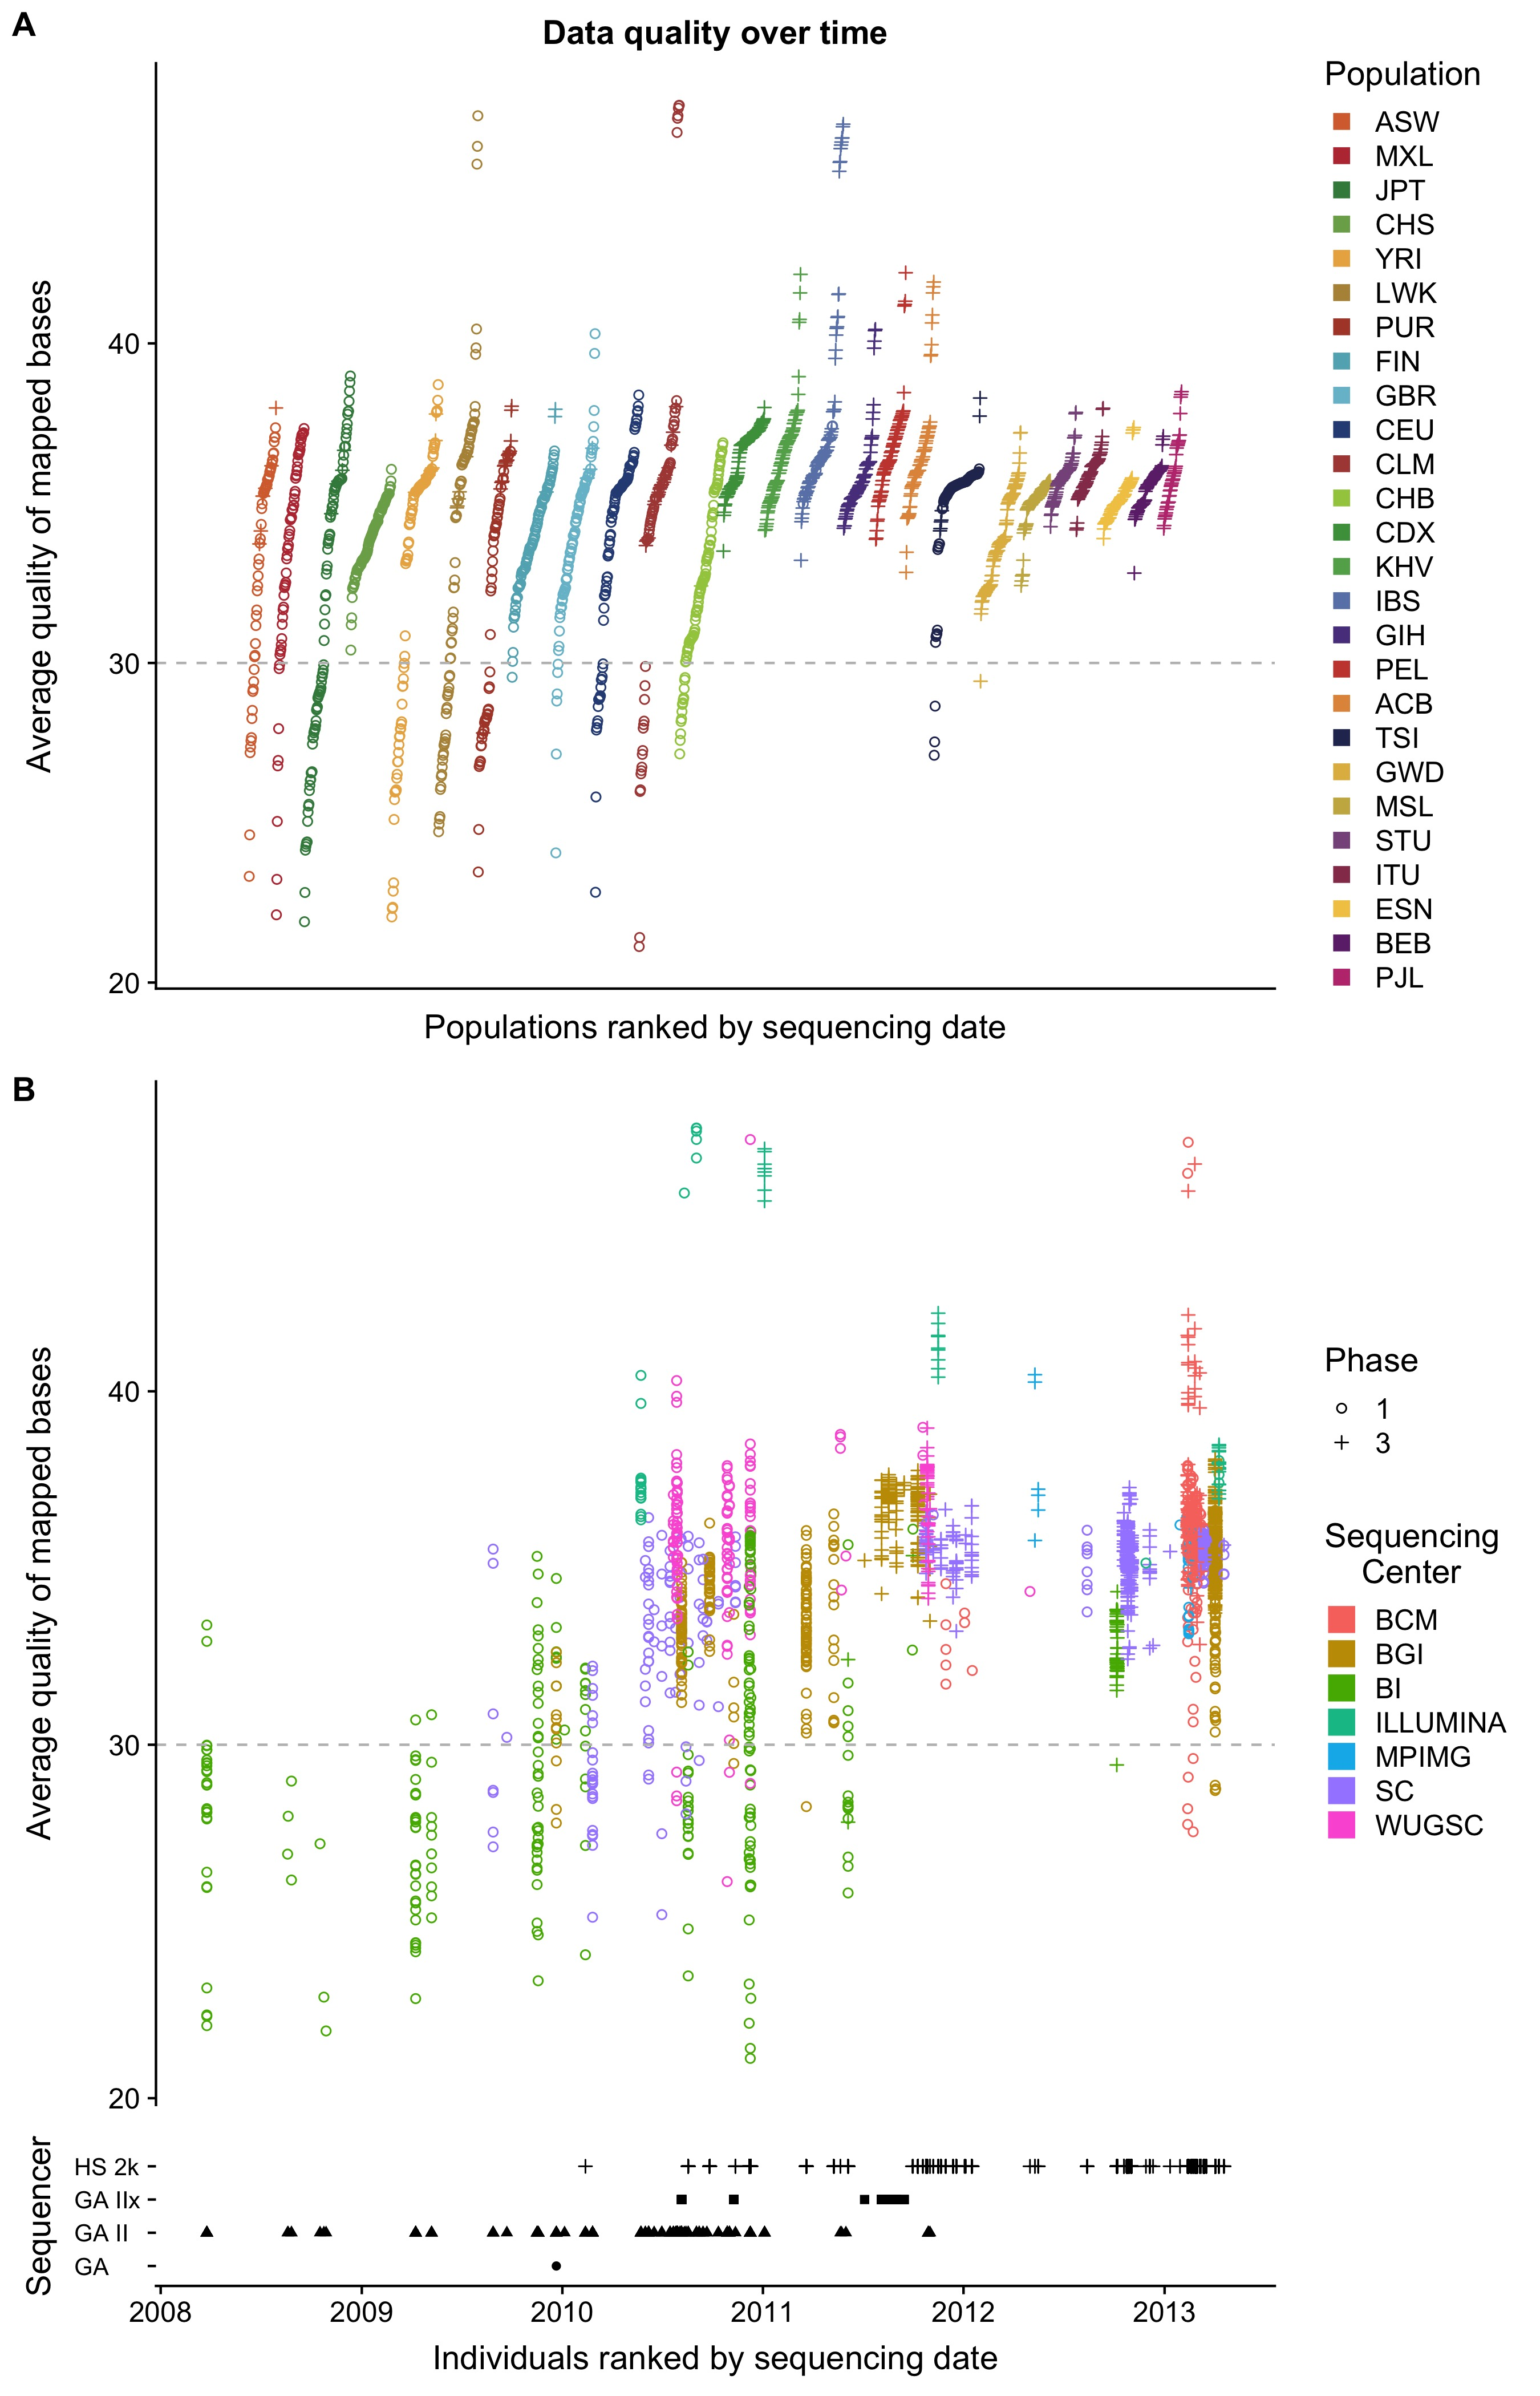
\includegraphics[width=0.75\hsize,keepaspectratio]{./Figures/MapQualOverTime.jpg}

\caption{\textbf{A} The average quality of mapped bases $Q$ for each individual per population included in the 1000 Genomes sequencing project. Individuals are ranked by the date of the earliest sequencing data is used for individuals sequenced more than once. The x-axis is ranked by the mean sequencing date per population. \textbf{B} The x-axis is sorted by the sequencing date per individual. The colors indicate the sequencing centres that produced the data for each individual and the shape indicates whether the individual belongs to Phase 1 or Phase 3 of the 1000 Genomes project. The bottom plot indicates the sequencing technologies used over time.}
\label{MapQual}
\end{center}
\end{figure}

\begin{figure}
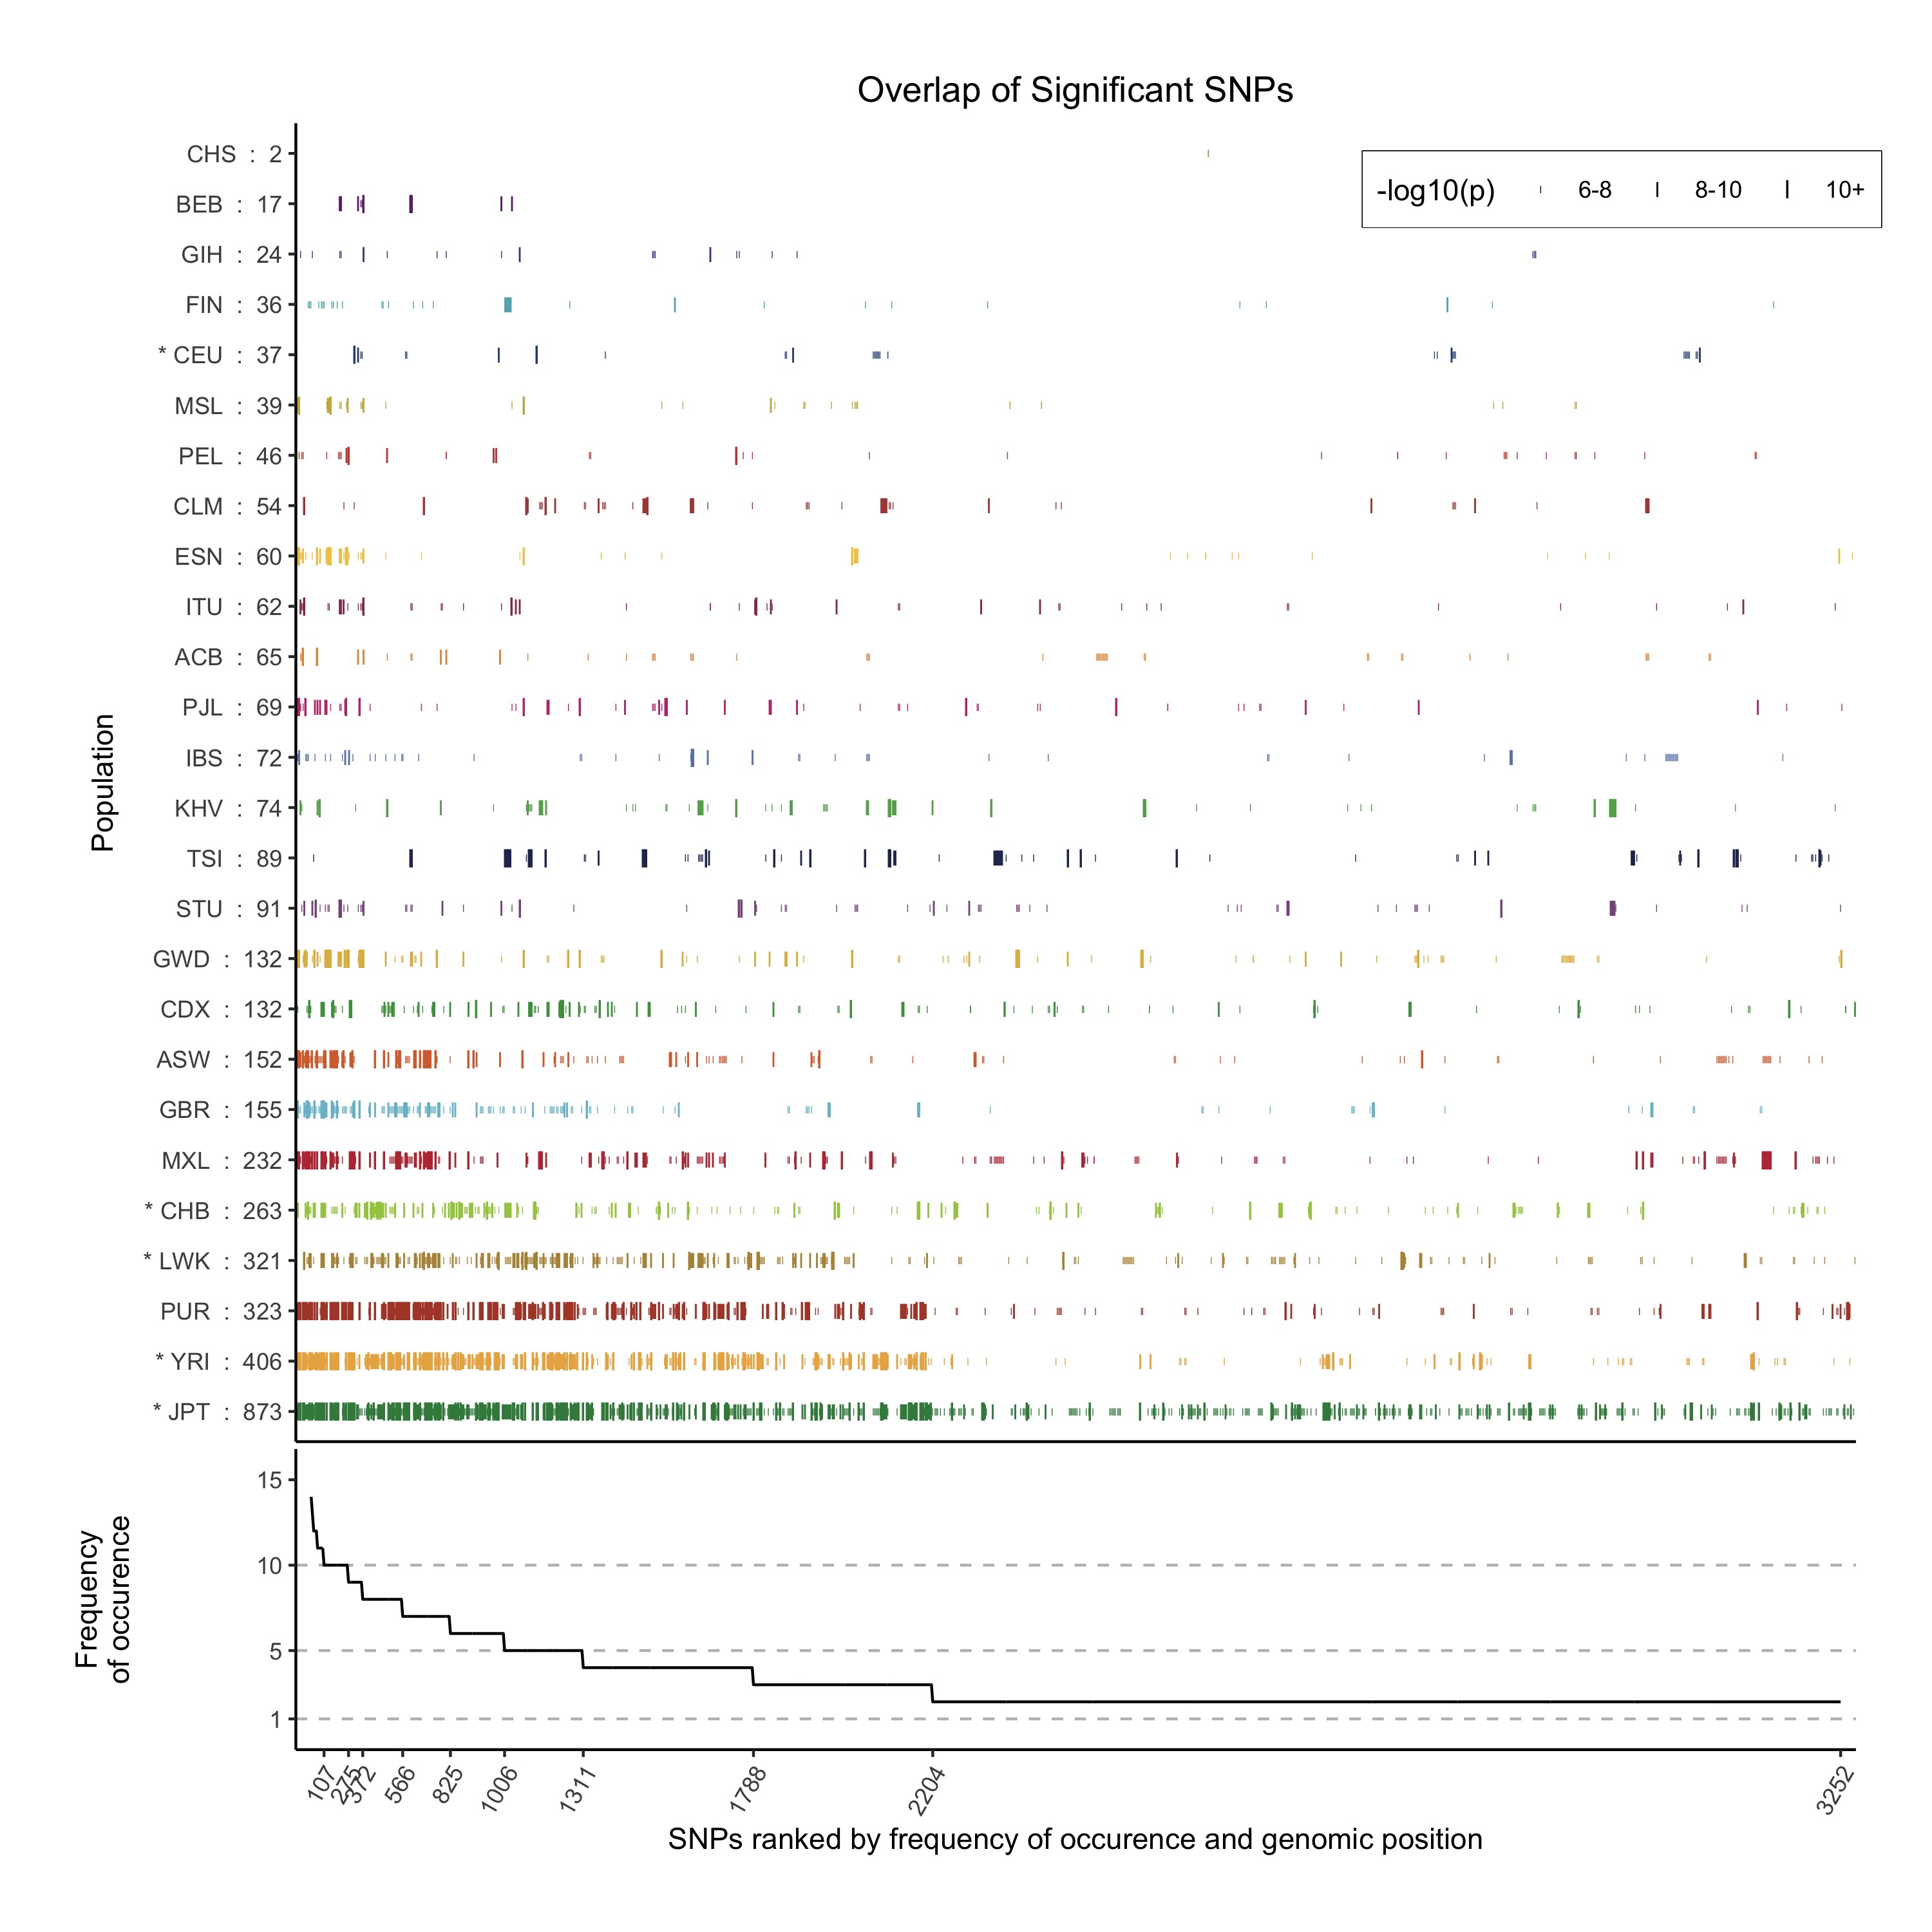
\includegraphics[width=\hsize,keepaspectratio]{./Figures/SNPOverlap6.jpg}

\caption{Overlap of SNPs identified independently to be associated with average quality of mapped bases $Q$.
The size of the crosses ( + ) are proportional to the -log10(p) value of that SNP.
The x axis is ranked by the frequency of occurrence of a SNP, then by genomic position.
Phase 1 populations are marked by a star ( * ).
The line plot underneath shows the number of populations for which a variant has reached significance.
The populations that tend to have the most individuals with low $Q$ also tend to have the most variants associated to $Q$. 
The same variants identified as being low quality independently in each population are found in other populations. }
  \label{OverLap}
\end{figure}

\begin{figure}
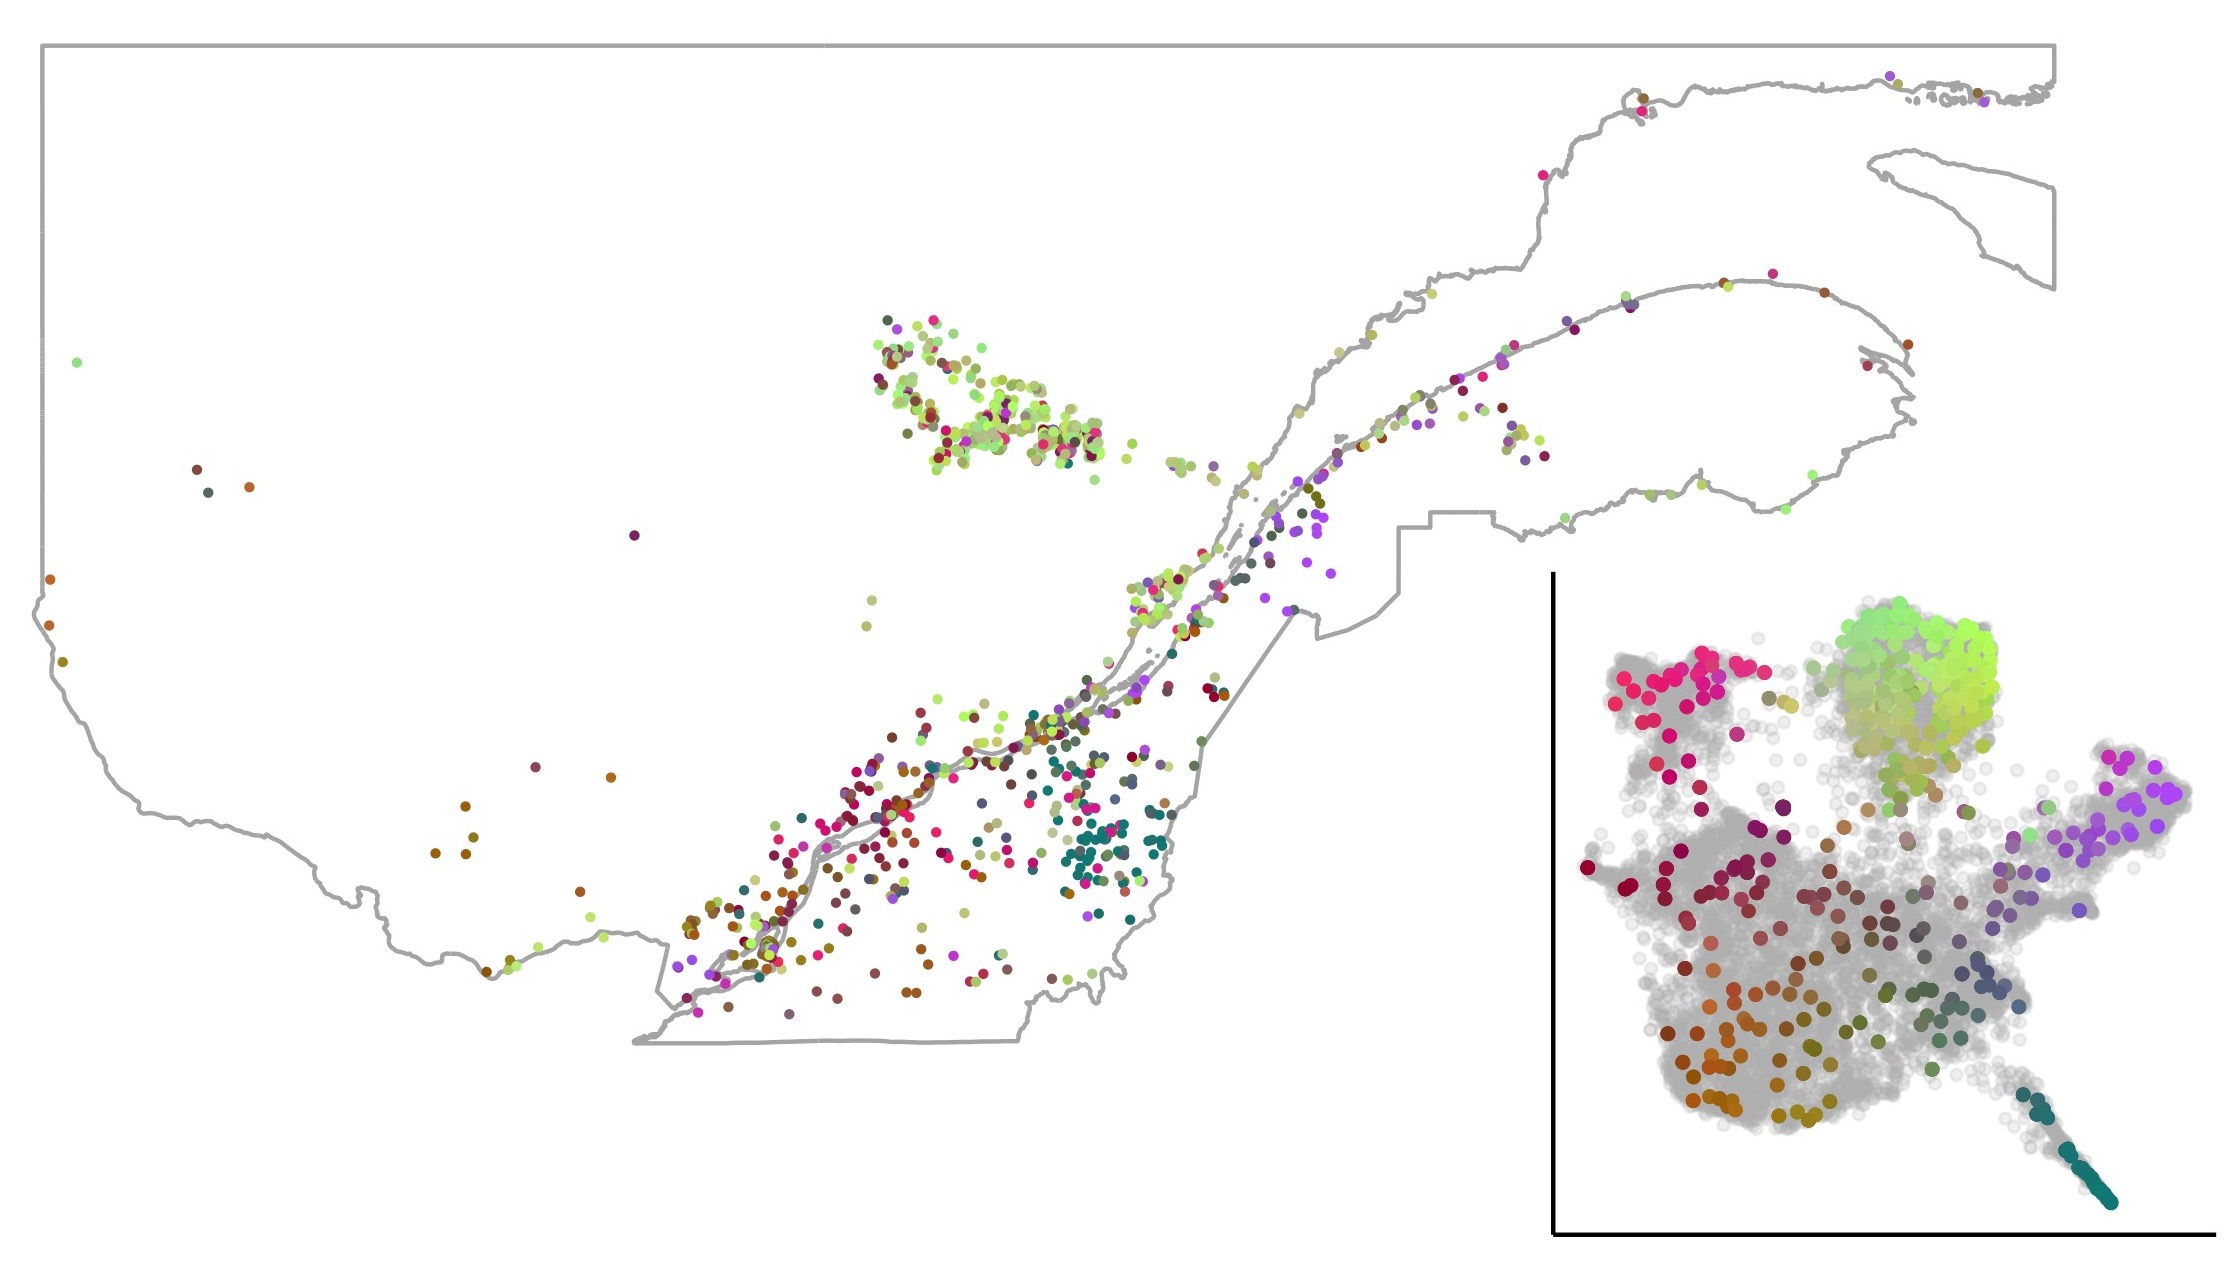
\includegraphics[width=\hsize,keepaspectratio]{./Figures/Genizon_BalSac_mapsInMaps4.jpg}

\caption{A map of Quebec colored by a 3D UMAP projection. 
The coloring of each individual is based on the three dimensional coordinates of the UMAP projection space (X,Y,Z) converted to three dimensional color space (R,G,B).
Therefore, Individuals with similar color are closer to each other in the projection.
Five genetic clusters are visible in the UMAP projection, these clusters also appear to be geographically linked. 
A flattened 2D view of of the 3D projection used for coloring is in the bottom right.}
\label{UMAP}
\end{figure}

\clearpage
%\begin{figure}
%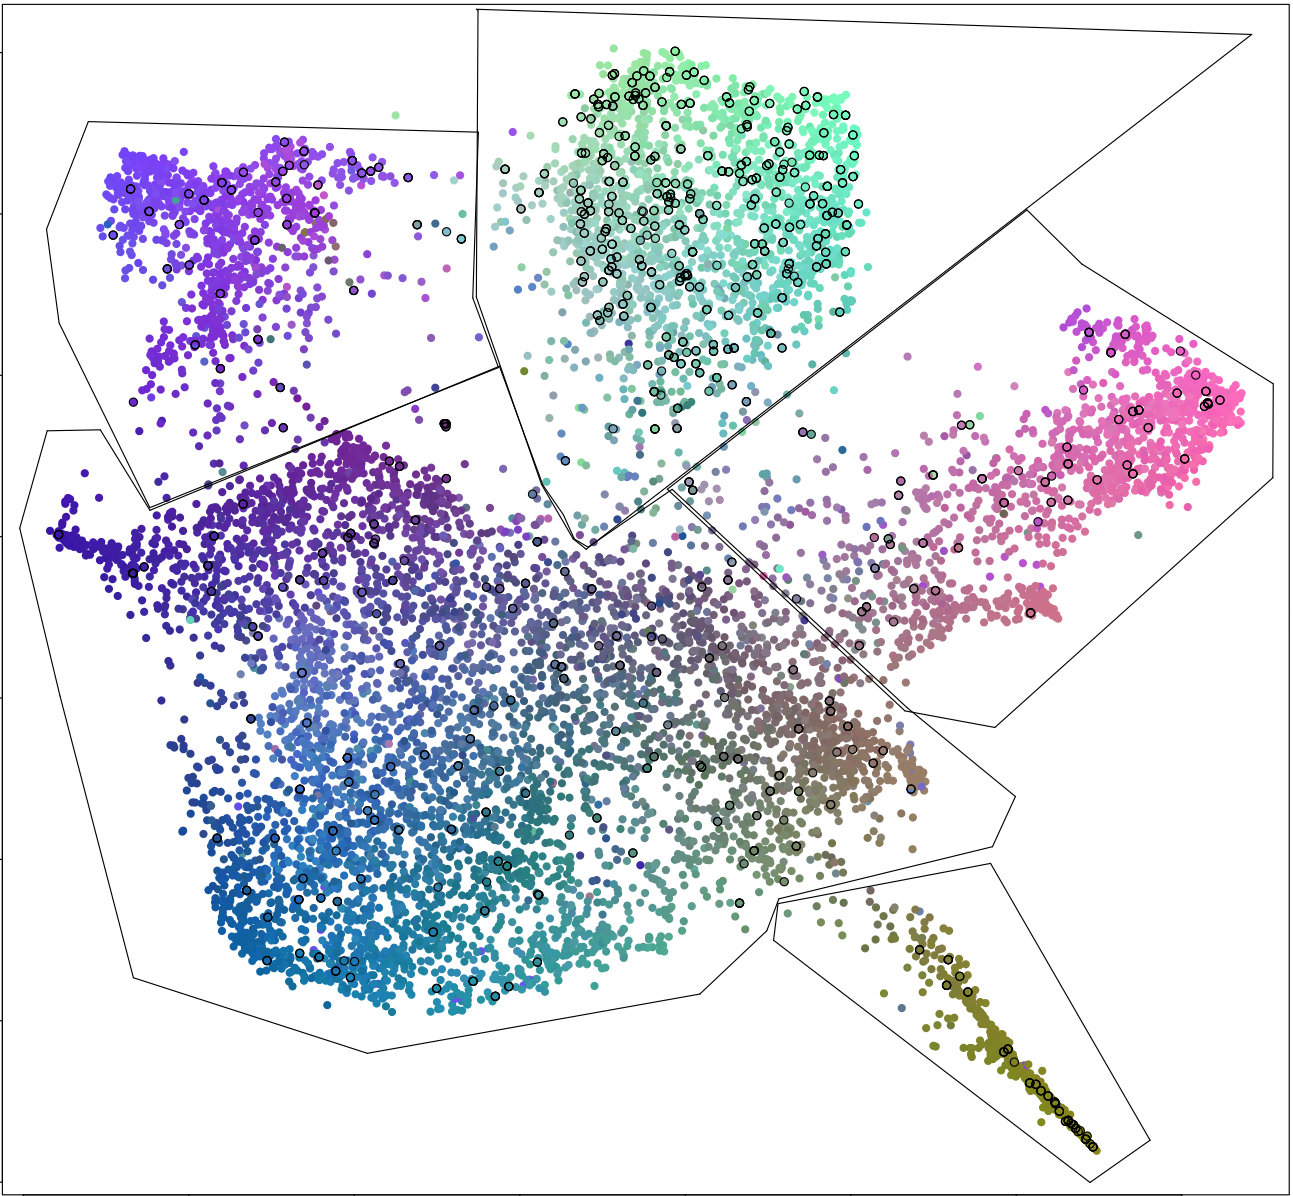
\includegraphics[width=\hsize,keepaspectratio]{./Figures/5Clusters.png}
%\label{Cluster}
%\end{figure}

% Include the appendices of the thesis as separate files from the Appendices folder
% Uncomment the lines as you write the Appendices

%\include{Appendices/AppendixA}


%----------------------------------------------------------------------------------------
%	BIBLIOGRAPHY
%----------------------------------------------------------------------------------------

\printbibliography[heading=bibintoc]

%----------------------------------------------------------------------------------------

\end{document}  
